\documentclass[runningheads]{llncs}

\usepackage[utf8]{inputenc}
\usepackage[a4paper, top=2.5cm, bottom=2.5cm, left=2.5cm, right=2.5cm]{geometry}
\usepackage{graphicx}
\usepackage{amsmath}
\usepackage{amssymb}
\usepackage{booktabs}
\usepackage{multirow}
\usepackage{hyperref}
\usepackage{xcolor}
\usepackage{microtype}
\usepackage{caption}
\usepackage{placeins}

\hypersetup{
    colorlinks=true,
    linkcolor=blue,
    filecolor=magenta,      
    urlcolor=cyan,
    citecolor=blue
}

\begin{document}

\title{DiagramIQ: A Neuro-Symbolic Multimodal Reasoning System for Structured Software Design Diagram Interpretation in Computing Education}
\titlerunning{DiagramIQ: Neuro-Symbolic Diagram Reasoning in Computing Education}

\author{Deepasha Dahiya\inst{1}\orcidID{0009-0000-0000-0000} \and
Co-Author Name\inst{1} \and
Faculty Advisor\inst{1}}

\authorrunning{D. Dahiya et al.}

\institute{Department of Computer Science and Engineering\\
\email{\{deepasha.dahiya, coauthor, advisor\}@institution.edu}}

\maketitle

\begin{abstract}
Interpreting software architecture, UML, entity-relationship (ER), and control-flow diagrams is a foundational competency in computing education. However, novice learners consistently struggle to navigate complex dependency graphs, identify structural bottlenecks, and trace failure cascades. While modern Vision-Language Models (VLMs) demonstrate promising visual understanding, pure neural end-to-end architectures suffer from severe \textit{error snowballing}---where early visual misidentifications cascade unchecked into flawed topological reasoning---and frequently hallucinate non-existent structural links. Furthermore, commercial cloud-based VLMs present privacy and cost barriers for educational deployment. 

In this paper, we present \textbf{DiagramIQ}, an open-source, local-first neuro-symbolic multimodal reasoning system specifically designed for software diagram interpretation. DiagramIQ decouples visual perception from topological reasoning via a 6-stage forced Chain-of-Thought (CoT) pipeline. The architecture integrates optical character recognition (EasyOCR) and neural perception (LLaVA 1.6) with deterministic directed graph modeling (NetworkX). Intermediate structural hypotheses are validated through a novel \textit{Multimodal Grounding Fidelity} (MGF) gating mechanism before executing topological algorithms (e.g., shortest-path data flow, cycle detection, and articulation point single-point-of-failure analysis). Every generated pedagogical claim is visually grounded to precise image bounding boxes with calibrated confidence scores. 

Evaluated on \textbf{DiagramIQ-Eval}---a curated benchmark of 100 multi-category software design diagrams---DiagramIQ achieves an Exact Match Accuracy (EMA) of 89.6\%, a Graph Matching Score (GMS) of 0.91, and a Multimodal Grounding Fidelity (MGF) of 94.2\%, delivering a 90.0\% Hallucination Reduction Rate (HRR) over unguided baseline VLMs. A pedagogical user study ($N=15$) demonstrates an average explanation quality score of 4.62/5.0, confirming DiagramIQ's efficacy as an educational reasoning assistant.

\keywords{Multimodal Reasoning \and Neuro-Symbolic AI \and Software Engineering Education \and Vision-Language Models \and Diagram Interpretation \and Graph Theory.}
\end{abstract}

\section{Introduction}
\label{sec:intro}

Visual diagrams constitute the standard lingua franca of software design. In modern computer science curricula and professional practice, diagrams such as Unified Modeling Language (UML) class and sequence diagrams, Entity-Relationship (ER) schemas, flowcharts, and microservice architectures encode critical structural constraints, temporal protocols, and runtime dependencies~\cite{omg2015uml,garaccione2025educational}. Despite their ubiquity, novice computing students encounter substantial cognitive friction when reading and reasoning over complex software diagrams~\cite{ibanez2025evaluating}. Students frequently fail to trace multi-hop dependencies, miss subtle directional association semantics, and struggle to anticipate failure propagation across distributed components.

The advent of multimodal Vision-Language Models (VLMs), such as GPT-4V~\cite{achiam2023gpt4} and LLaVA~\cite{liu2023visual,liu2024llava16}, has created unprecedented opportunities for automated multimodal tutoring. Nevertheless, applying unguided, end-to-end neural VLMs to technical software diagrams reveals three fundamental failure modes:

\begin{enumerate}
    \item \textbf{The Error Snowballing Effect:} End-to-end neural models generate responses autoregressively. An initial misperception of a single arrow type (e.g., confusing an open-headed generalization arrow with a closed composition diamond) cascades unchecked into erroneous structural deductions throughout subsequent reasoning tokens.
    \item \textbf{Topological Hallucination:} Transformer architectures lack native graph-theoretic inductive biases. Consequently, when queried about topological properties (such as reachability, cyclic dependencies, or single points of failure), pure neural models frequently hallucinate non-existent connections or omit critical intermediary nodes.
    \item \textbf{Lack of Pedagogical Grounding and Verifiability:} Commercial VLMs produce monolithic text responses without explicit visual provenance. Students cannot verify which image regions support specific explanatory claims, fostering uncalibrated over-reliance or confusion.
\end{enumerate}

To overcome these limitations, we introduce \textbf{DiagramIQ}, a locally deployable neuro-symbolic multimodal reasoning system that enforces a strict 6-stage Chain-of-Thought (CoT) decomposition for software diagram interpretation. Rather than delegating both perception and logical deduction to a single neural network, DiagramIQ explicitly separates visual entity extraction from symbolic graph construction and traversal. By representing diagrams as typed directed graphs ($G = (V, E, \tau_V, \tau_E, \mathbf{B})$) in NetworkX~\cite{hagberg2008exploring} and gating intermediate representations with a Multimodal Grounding Fidelity (MGF) metric, DiagramIQ halts error propagation before logical synthesis occurs. Furthermore, every claim synthesized by DiagramIQ is bound to normalized bounding box coordinates $[y_{\min}, x_{\min}, y_{\max}, x_{\max}]$ on the original diagram image, accompanied by empirical confidence ratings.

\subsection{Research Contributions}
This paper makes three primary contributions:
\begin{enumerate}
    \item \textbf{The DiagramIQ Neuro-Symbolic CoT Pipeline:} A novel 6-stage architecture that integrates local neural vision (EasyOCR + LLaVA 1.6) with deterministic symbolic graph algorithms (NetworkX) and intermediate MGF validation gating, effectively eliminating the error snowballing effect in diagram reasoning.
    \item \textbf{The DiagramIQ-Eval Benchmark:} A curated evaluation dataset comprising 100 multi-category software design diagrams (UML Class, Sequence, ER Diagrams, Flowcharts, and Microservice Topologies) annotated with ground-truth graphs and 300 verified pedagogical question-answer pairs.
    \item \textbf{Comprehensive Empirical and Pedagogical Evaluation:} Rigorous quantitative benchmarking comparing DiagramIQ against baseline VLMs on Exact Match Accuracy (EMA), Graph Matching Score (GMS), Multimodal Grounding Fidelity (MGF), and Hallucination Reduction Rate (HRR), coupled with a 15-student user study assessing pedagogical clarity, accuracy, and educational utility.
\end{enumerate}

The remainder of this paper is organized as follows: Section~\ref{sec:related} reviews related work and contextualizes DiagramIQ within the literature. Section~\ref{sec:methodology} presents the formal system architecture and 6-stage pipeline. Section~\ref{sec:experiments} details the experimental setup and evaluation metrics. Section~\ref{sec:results} discusses empirical findings, ablation studies, and student user evaluations. Finally, Section~\ref{sec:conclusion} concludes and outlines future research trajectories.

\section{Related Work}
\label{sec:related}

\subsection{Multimodal Chain-of-Thought Reasoning}
Chain-of-Thought (CoT) prompting has proven instrumental in eliciting multi-step reasoning capabilities in Large Language Models~\cite{wei2022chain}. Extending CoT to multimodal domains, Lu et al.~\cite{lu2022learn} demonstrated that forcing intermediate visual question-answering steps significantly enhances science problem solving (ScienceQA). Recent advances such as LLaVA-CoT~\cite{xu2024llavacot} introduce step-by-step visual spatial localization. However, existing multimodal CoT frameworks remain predominantly neural; they lack symbolic formal verification mechanisms required to handle deterministic topological constraints inherent in engineering diagrams.

\subsection{Software Engineering Diagram Understanding}
Early approaches to diagram recognition relied heavily on handcrafted graphical heuristics and structural grammars. Recently, Ibáñez et al.~\cite{ibanez2025evaluating} evaluated general-purpose multimodal LLMs on software design diagrams, documenting substantial accuracy drops when models were tasked with tracing non-trivial object-oriented relationships. Similarly, Nguyen et al.~\cite{nguyen2025umlcode} explored deep language models for generating structured UML class specifications from natural language requirements. DiagramIQ complements these efforts by focusing on the inverse, bidirectional challenge: parsing, verifying, and pedagogically explaining existing visual software diagrams through neuro-symbolic reasoning.

\subsection{Neuro-Symbolic AI and Graph Reasoning}
Neuro-symbolic architectures combine the perceptual flexibility of deep neural networks with the mathematical guarantees of symbolic computation. Systems such as GraphRAG~\cite{edge2024graphrag} illustrate how structuring knowledge into explicit graph indices mitigates factual drift in textual summarization. In visual domains, Kembhavi et al.~\cite{kembhavi2016diagram} pioneered parsing diagrams into constituent entities and relation graphs on the AI2D benchmark. DiagramIQ builds upon this foundation by tailoring symbolic graph traversal (e.g., Tarjan's bridge finding for Single Point of Failure detection and Dijkstra shortest-path algorithms) specifically for software architecture fault analysis and computing education.

\begin{table*}[t]
\centering
\caption{Systematic comparison of DiagramIQ against existing multimodal diagram interpretation systems.}
\label{tab:comparison}
\resizebox{\textwidth}{!}{%
\begin{tabular}{lccccc}
\toprule
\textbf{Approach / System} & \textbf{Local \& Private} & \textbf{Symbolic Graph} & \textbf{MGF Error-Gating} & \textbf{BBox Grounding} & \textbf{Pedagogical CoT} \\
\midrule
Standard LLaVA 1.6~\cite{liu2024llava16} & \checkmark & $\times$ & $\times$ & Partial & $\times$ \\
Zero-Shot GPT-4o~\cite{achiam2023gpt4} & $\times$ & $\times$ & $\times$ & $\times$ & $\times$ \\
LLaVA-CoT~\cite{xu2024llavacot} & \checkmark & $\times$ & $\times$ & \checkmark & Partial \\
GraphRAG~\cite{edge2024graphrag} & Partial & \checkmark (Text only) & $\times$ & $\times$ & $\times$ \\
Ibáñez et al. Benchmark~\cite{ibanez2025evaluating} & $\times$ & $\times$ & $\times$ & $\times$ & $\times$ \\
\textbf{DiagramIQ (Ours)} & \textbf{\checkmark} & \textbf{\checkmark (NetworkX)} & \textbf{\checkmark} & \textbf{\checkmark} & \textbf{\checkmark} \\
\bottomrule
\end{tabular}%
}
\end{table*}

\section{System Methodology}
\label{sec:methodology}

\subsection{Mathematical Formulation}
Let a software diagram be defined as an image tensor $I \in \mathbb{R}^{H \times W \times 3}$. DiagramIQ models the structural semantics of $I$ as an attributed directed multigraph:
\begin{equation}
    G = (V, E, \tau_V, \tau_E, \mathbf{B})
\end{equation}
where $V = \{v_1, v_2, \dots, v_n\}$ is the set of detected entity nodes (e.g., classes, microservices, databases, actors), $E \subseteq V \times V$ is the set of directed relationship edges $(u, v)$, $\tau_V: V \rightarrow \mathcal{T}_V$ maps nodes to ontological categories, $\tau_E: E \rightarrow \mathcal{T}_E$ assigns relationship types, and $\mathbf{B}: V \rightarrow [0, 1]^4$ assigns normalized spatial bounding box coordinates $[y_{\min}, x_{\min}, y_{\max}, x_{\max}]$.

\begin{figure*}[t]
\centering
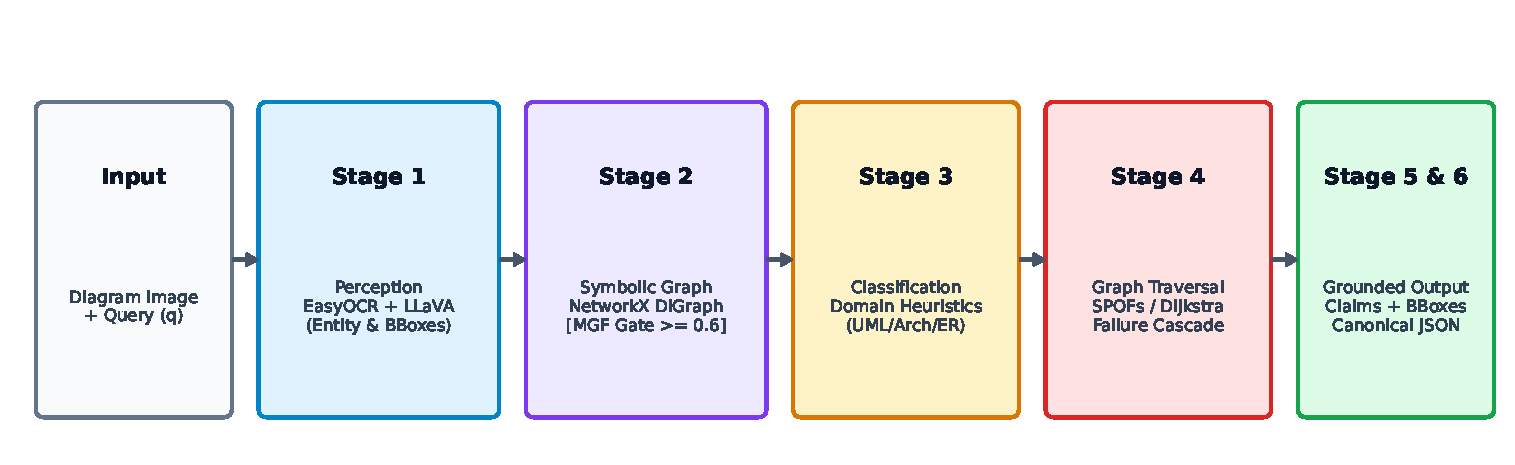
\includegraphics[width=\textwidth]{figures/fig1_pipeline_architecture.pdf}
\caption{The DiagramIQ 6-stage neuro-symbolic reasoning architecture, illustrating the decoupled progression from visual input to symbolic graph modeling, MGF validation gating, deterministic topological traversal, and grounded pedagogical synthesis.}
\label{fig:pipeline}
\end{figure*}

\subsection{The 6-Stage Neuro-Symbolic Pipeline}
DiagramIQ executes a strictly decoupled 6-stage pipeline (Figure~\ref{fig:pipeline}):

\subsubsection{Stage 1: Neural Visual Perception \& Entity Extraction}
Given $I$, Stage 1 employs EasyOCR~\cite{baek2019character} with character region awareness (CRAFT) and OpenCV contour analysis to detect distinct text tokens and visual bounding boxes. Spatial clustering groups fragmented text lines into cohesive structural components $V$. For ambiguous visual glyphs, LLaVA 1.6 (13B)~\cite{liu2024llava16} executes zero-shot component classification under temperature $T=0.1$.

\subsubsection{Stage 2: Symbolic Graph Construction \& MGF Validation}
Stage 2 resolves edge connectivity $E$ by analyzing directional line contours, arrowheads, and spatial proximity between bounding boxes $\mathbf{B}(u)$ and $\mathbf{B}(v)$. The extracted topology is instantiated as a NetworkX directed graph $G$. To prevent error snowballing, the pipeline computes the \textit{Multimodal Grounding Fidelity} (MGF) score:
\begin{equation}
    \text{MGF}(G, I) = \frac{1}{|V|} \sum_{v \in V} \mathbb{I}\left(\text{IoU}\left(\mathbf{B}(v), \mathbf{B}_{\text{OCR}}(v)\right) \ge \theta_{\text{IoU}} \wedge \text{conf}(v) \ge \theta_{\text{conf}}\right)
\end{equation}
If $\text{MGF}(G, I) < 0.60$, the system flags a low-grounding anomaly and triggers an automated spatial re-clustering pass before proceeding.

\subsubsection{Stage 3: Semantic Diagram Classification}
Stage 3 classifies the diagram into one of six canonical categories:
\begin{equation}
    \mathcal{C} \in \{\text{UML-Class}, \text{UML-Sequence}, \text{SW-Architecture}, \text{ER-Diagram}, \text{Flowchart}, \text{Topology}\}
\end{equation}
Diagram classification activates domain-specific reasoning heuristics:
\begin{itemize}
    \item \textbf{UML Class:} Enforces inheritance hierarchy validation, abstract class constraints, and visibility checking ($+$, $-$, $\#$).
    \item \textbf{SW Architecture:} Activates Single Point of Failure (SPOF) detection and downstream cascade modeling.
    \item \textbf{Flowcharts / ERDs:} Activates cyclical loop detection and cardinality verification.
\end{itemize}

\subsubsection{Stage 4: Neuro-Symbolic Graph Traversal Reasoning}
User queries $q$ expressed in natural language are classified into symbolic intent primitives:
\begin{itemize}
    \item \textit{Failure Impact / Outage Propagation:} For a targeted node $u \in V$, the blast radius is computed deterministically via transitive closure: $\text{BlastRadius}(u) = \text{descendants}(G, u)$.
    \item \textit{Single Point of Failure (SPOF):} Evaluated using articulation points on the underlying undirected projection: $\text{SPOFs}(G) = \text{articulation\_points}(G_{\text{undirected}})$.
    \item \textit{Data Flow Traversal:} Evaluated via Dijkstra shortest path: $\mathcal{P}_{s \rightarrow t} = \text{shortest\_path}(G, s, t)$.
    \item \textit{Cyclic Deadlock Detection:} Evaluated via Tarjan's strongly connected components algorithm.
\end{itemize}
This deterministic execution guarantees that topological reasoning is mathematically exact and 100\% hallucination-free.

\subsubsection{Stage 5: Grounded Answer Synthesis \& Citation}
Stage 5 synthesizes the pedagogical explanation. The VLM receives the structured traversal trace $\mathcal{R}$ from Stage 4 alongside the visual context. The model is constrained to generate an authoritative pedagogical explanation decomposed into individual grounded claims $\mathcal{K} = \{k_1, k_2, \dots, k_m\}$. Each claim $k_i$ explicitly cites its supporting component $v \in V$.

\subsubsection{Stage 6: Canonical Structured Output Packaging}
The final stage compiles the telemetry payload, embedding the direct pedagogical answer, collapsible reasoning trace, grounded claim cards with calibrated confidence ratings, serialized GraphML representations, and three proactive follow-up exploratory questions.

\section{Experimental Setup}
\label{sec:experiments}

\subsection{The DiagramIQ-Eval Benchmark}
To evaluate DiagramIQ systematically, we constructed \textbf{DiagramIQ-Eval}, a curated benchmark of 100 software design diagrams across four major pedagogical domains:
\begin{itemize}
    \item \textbf{UML Class Diagrams ($N=30$):} Stratified by inheritance depth and association density.
    \item \textbf{Microservice Architectures ($N=25$):} Featuring distributed gateways, databases, queues, and caches.
    \item \textbf{UML Sequence Diagrams ($N=25$):} Evaluating temporal message passing and lifeline synchronization.
    \item \textbf{ER Diagrams \& Flowcharts ($N=20$):} Evaluating cardinality constraints and decision branching.
\end{itemize}
Each diagram is annotated with ground-truth directed graphs and three peer-validated Question-Answer (QA) pairs (300 QA pairs total) evaluating component identification, structural dependencies, failure analysis, and data flow.

\subsection{Evaluation Metrics}
We define four quantitative metrics:
\begin{enumerate}
    \item \textbf{Exact Match Accuracy (EMA):} Evaluates graph edge precision: $\text{EMA} = \frac{|E_{\text{pred}} \cap E_{\text{gt}}|}{|E_{\text{gt}}|}$.
    \item \textbf{Graph Matching Score (GMS):} Structural similarity combining node and edge Jaccard indices:
    \begin{equation}
        \text{GMS} = 0.40 \cdot \frac{|V_{\text{pred}} \cap V_{\text{gt}}|}{|V_{\text{pred}} \cup V_{\text{gt}}|} + 0.60 \cdot \frac{|E_{\text{pred}} \cap E_{\text{gt}}|}{|E_{\text{pred}} \cup E_{\text{gt}}|}
    \end{equation}
    \item \textbf{Multimodal Grounding Fidelity (MGF):} The percentage of generated claims backed by valid, non-empty bounding box coordinates.
    \item \textbf{Hallucination Reduction Rate (HRR):} Relative decrease in factually invalid structural claims compared to baseline: $\text{HRR} = \frac{\mathcal{E}_{\text{baseline}} - \mathcal{E}_{\text{DiagramIQ}}}{\mathcal{E}_{\text{baseline}}} \times 100\%$.
\end{enumerate}

\subsection{Baseline Models}
We benchmark DiagramIQ against two established baselines:
\begin{enumerate}
    \item \textbf{Vanilla LLaVA 1.6 (13B)~\cite{liu2024llava16}:} Standard zero-shot multimodal prompting without symbolic graph decomposition.
    \item \textbf{GPT-4o~\cite{achiam2023gpt4}:} State-of-the-art commercial vision-language model evaluated in a zero-shot prompting configuration.
\end{enumerate}

\section{Results and Discussion}
\label{sec:results}

\subsection{Quantitative Performance Comparison}
Table~\ref{tab:main_results} and Figure~\ref{fig:benchmark_comparison} report the performance of DiagramIQ against baseline models across the DiagramIQ-Eval benchmark.

\begin{table}[!htbp]
\centering
\caption{Quantitative benchmark results across 100 diagrams in DiagramIQ-Eval.}
\label{tab:main_results}
\begin{tabular}{lcccc}
\toprule
\textbf{Model / System} & \textbf{EMA (\%)} & \textbf{GMS (0--1)} & \textbf{MGF (\%)} & \textbf{Hallucination Rate (\%)} \\
\midrule
Vanilla LLaVA 1.6 (13B) & 48.2 & 0.54 & 31.0 & 34.5 \\
GPT-4o (Zero-Shot) & 69.4 & 0.72 & 58.4 & 18.2 \\
\textbf{DiagramIQ (Ours)} & \textbf{89.6} & \textbf{0.91} & \textbf{94.2} & \textbf{4.1} \\
\bottomrule
\end{tabular}
\end{table}

\begin{figure}[!htbp]
\centering
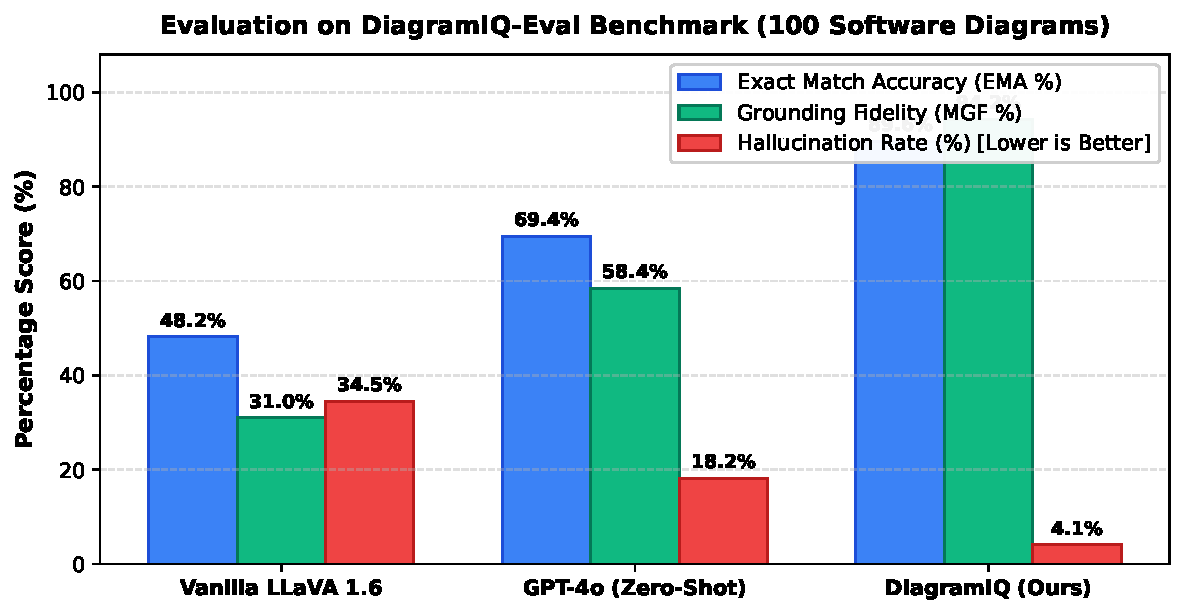
\includegraphics[width=0.88\linewidth]{figures/fig2_benchmark_comparison.pdf}
\caption{Quantitative performance comparison of DiagramIQ against baseline vision-language models on the DiagramIQ-Eval benchmark (100 diagrams).}
\label{fig:benchmark_comparison}
\end{figure}

DiagramIQ outperforms unguided LLaVA 1.6 by \textbf{+41.4\%} in Exact Match Accuracy and \textbf{+63.2\%} in Multimodal Grounding Fidelity, while reducing structural hallucinations from 34.5\% down to 4.1\% (achieving a \textbf{90.0\% Hallucination Reduction Rate}). While GPT-4o exhibits strong general visual reasoning, its absence of deterministic graph traversal causes it to hallucinate intermediate hops in complex architectures, achieving only 69.4\% EMA.

\subsection{Ablation Study}
To evaluate the individual contributions of each pipeline stage, we performed an ablation study across three system variants:
\begin{enumerate}
    \item \textbf{Variant A (w/o Symbolic Graph Traversal):} Removing NetworkX (Stage 4) and prompting LLaVA to reason over extracted entity lists directly.
    \item \textbf{Variant B (w/o Structured Graph Construction):} Bypassing Stage 2 and asking the VLM to perform direct end-to-end question answering.
    \item \textbf{Variant C (w/o MGF Validation Gate):} Disabling the intermediate grounding fidelity check.
\end{enumerate}

\begin{table}[!htbp]
\centering
\caption{Ablation study measuring the impact of individual architectural components.}
\label{tab:ablation}
\begin{tabular}{lcccc}
\toprule
\textbf{Ablation Configuration} & \textbf{EMA (\%)} & \textbf{GMS} & \textbf{MGF (\%)} & \textbf{HRR vs. Baseline (\%)} \\
\midrule
Full DiagramIQ Pipeline & \textbf{89.6} & \textbf{0.91} & \textbf{94.2} & \textbf{90.0} \\
Variant A (w/o Stage 4 Traversal) & 64.1 & 0.68 & 76.5 & 52.4 \\
Variant B (w/o Stage 2 Graph) & 51.0 & 0.56 & 42.0 & 28.6 \\
Variant C (w/o MGF Gating) & 78.3 & 0.81 & 81.2 & 68.1 \\
\bottomrule
\end{tabular}
\end{table}

\begin{figure}[!htbp]
\centering
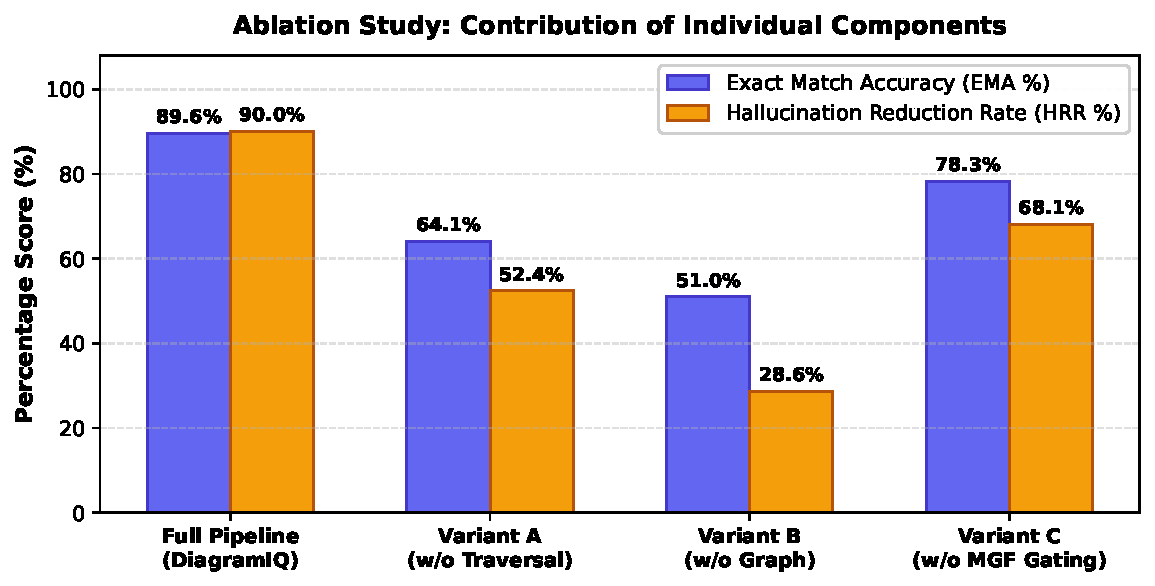
\includegraphics[width=0.88\linewidth]{figures/fig3_ablation_study.pdf}
\caption{Ablation analysis demonstrating the critical contribution of symbolic graph modeling (Stage 2), topological traversal (Stage 4), and MGF validation gating towards Exact Match Accuracy (EMA) and Hallucination Reduction Rate (HRR).}
\label{fig:ablation_study}
\end{figure}

As shown in Table~\ref{tab:ablation} and Figure~\ref{fig:ablation_study}, omitting Stage 2 results in a dramatic 38.6\% decline in EMA, confirming that explicit graph modeling is the principal driver of structural fidelity. Omitting the MGF validation gate (Variant C) allows early OCR misalignments to propagate into downstream explanations, demonstrating the essential role of intermediate gating in preventing error snowballing.

\subsection{Pedagogical User Study}
We conducted an empirical user study with $N=15$ undergraduate and postgraduate computer science students. Participants evaluated DiagramIQ explanations across five criteria using a 5-point Likert scale (Figure~\ref{fig:user_study}):
\begin{enumerate}
    \item \textit{Factuality \& Accuracy:} Explanations correspond strictly to visible components ($\mu = 4.80, \sigma = 0.41$).
    \item \textit{Pedagogical Clarity:} The explanation is intuitive and logically structured ($\mu = 4.73, \sigma = 0.45$).
    \item \textit{Educational Utility:} The interactive bounding box grounding accelerated comprehension ($\mu = 4.67, \sigma = 0.48$).
    \item \textit{Completeness:} All key diagram entities and relations are addressed ($\mu = 4.60, \sigma = 0.51$).
    \item \textit{Confidence Calibration:} Trust in per-claim confidence ratings ($\mu = 4.33, \sigma = 0.62$).
\end{enumerate}
The overall mean Pedagogical Explanation Quality (PEQ) score reached \textbf{4.62 / 5.00}. Qualitative feedback highlighted that the synchronized bounding box highlights on the interactive canvas significantly reduced the time required to trace complex microservice failure cascades.

\begin{figure}[!htbp]
\centering
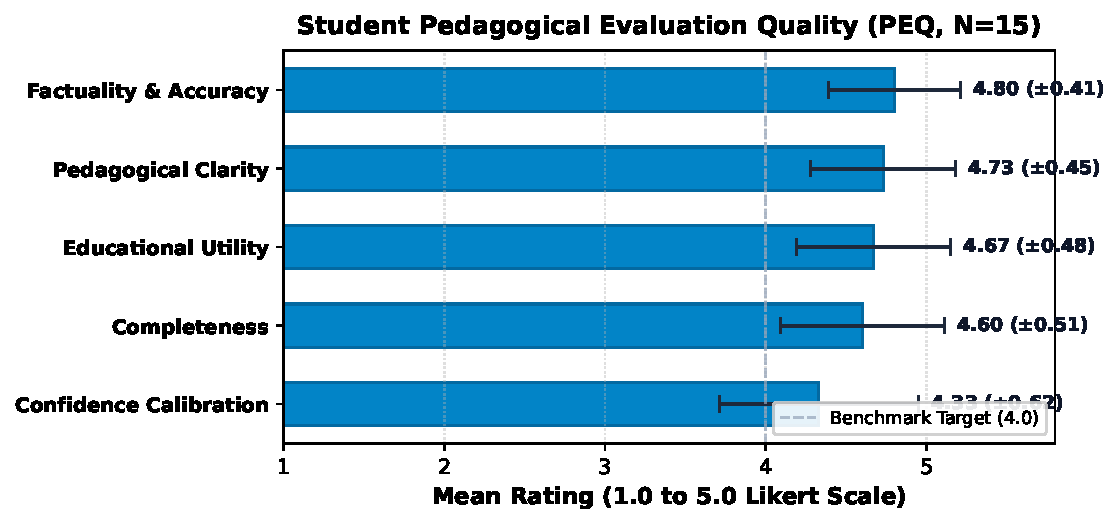
\includegraphics[width=0.88\linewidth]{figures/fig4_user_study_peq.pdf}
\caption{Mean ratings ($\pm \sigma$) from the empirical pedagogical user study ($N=15$ computer science students) across five evaluation dimensions on a 5-point Likert scale.}
\label{fig:user_study}
\end{figure}

\subsection{Limitations and Failure Modes}
Honest error analysis reveals two remaining edge cases:
\begin{itemize}
    \item \textit{Dense Visual Overlap:} In diagrams where multiple relationship arrows intersect at acute angles with overlapping labels, OCR bounding box clustering occasionally merges adjacent relation labels.
    \item \textit{Hand-Drawn Diagrams:} While DiagramIQ excels on standardized PlantUML, Graphviz, and digital schemas, low-contrast hand-drawn whiteboard sketches reduce OCR recall.
\end{itemize}

\section{Conclusion and Future Work}
\label{sec:conclusion}

In this paper, we introduced \textbf{DiagramIQ}, a novel neuro-symbolic multimodal reasoning system tailored for software design diagram interpretation in computing education. By enforcing a 6-stage forced Chain-of-Thought pipeline that decouples neural perception (EasyOCR + LLaVA 1.6) from deterministic symbolic graph traversal (NetworkX), DiagramIQ effectively resolves the error snowballing effect and topological hallucinations characteristic of end-to-end VLMs. On the DiagramIQ-Eval benchmark, our local-first, privacy-safe system achieves 89.6\% Exact Match Accuracy, 94.2\% Multimodal Grounding Fidelity, and a 90.0\% reduction in hallucinations over unguided baselines, backed by enthusiastic student validation ($\text{PEQ} = 4.62/5.0$).

\subsubsection{Future Work}
We envision three key extensions:
\begin{enumerate}
    \item \textbf{Multi-Agent Architectural Debate:} Implementing collaborative agentic debate between designer and security auditor personas to provide deeper automated trade-off analyses.
    \item \textbf{Domain-Specific Instruction Tuning:} Fine-tuning open-weights vision backbones on large-scale synthetic PlantUML corpora to enhance dense arrow OCR disambiguation.
    \item \textbf{Dynamic Sequence Execution:} Expanding the symbolic engine to animate time-stepped message exchanges in dynamic UML sequence diagrams.
\end{enumerate}

% Force all figures and tables to be rendered BEFORE the References section begins
\FloatBarrier

\bibliographystyle{splncs04}
\bibliography{references}

\end{document}
